\documentclass[8pt,aspectratio=169]{beamer}
\usetheme{Boadilla}

\usepackage{hyperref}
\usepackage{graphicx}
\usepackage{subfig}
\usepackage{amsmath,amssymb}

\graphicspath{ {images/} }

\usepackage{tikz}

%Some useful commands for QM
\newcommand{\bra}[1]{\left< #1 \right|}
\newcommand{\ket}[1]{\left| #1 \right>}
\newcommand{\expVal}[1]{\left< #1 \right>}
\newcommand{\braket}[2]{\left<#1|#2\right>}

%Stolen from http://tex.stackexchange.com/questions/178800/creating-sections-each-with-title-pages-in-beamers-slides
\AtBeginSection[]{
  \begin{frame}
  \vfill
  \centering
  \begin{beamercolorbox}[sep=8pt,center,shadow=true,rounded=true]{title}
    \usebeamerfont{title}\insertsectionhead\par%
  \end{beamercolorbox}
  \vfill
  \end{frame}
}

\title{Holographic Complexity in Non-Commutative Gauge Theory}
\subtitle{Work with Stefan Eccles, Willy Fischler, and Ming-Lei Xiao\\ arxiv:1710.07833}
\author{Josiah Couch}
\institute{University of Texas at Austin}
\date{23 March 2018}



\begin{document}

\begin{frame}
\titlepage\end{frame}

%\begin{frame}
%\frametitle{Outline}
%\tableofcontents[]
%\end{frame}

%\section{Introduction}

%\begin{frame}
%\frametitle{Introduction}

%Given the recent interest in the holographic complexity conjectures, it is interesting to test these conjectures in new contexts, to see if they hold up under closer scrutiny. With this in mind, we will examine holographic complexity in a geometry dual to non-commutative super Yang-Mills at finite temperature. In particular, we will be interested in the behavior of the complexity as we vary the Moyal scale of the boundary theory. In the limit where the Moyal scale is sent to zero, we will recover the usual result for a planar black hole in AdS$_5$. On the other hand, as we make the Moyal scale large, we find that we get an enhancement of the late time complexification rate, which asympototes to an enhancement.

%\end{frame}

\begin{frame}
\frametitle{Introduction}

In this talk, we will consider the growth rate of holographic complexity in a geometry dual to non-commutative super Yang-Mills (NCSYM), according to 'complexity = action'. A brief outline is as follows:

\begin{itemize}

\item First, we will recall the holographic complexity conjectures, in particular 'complexity = action', or CA.

\item Next, we will briefly discuss the geometry dual to ($\mathcal{N} = 4$) NCSYM.

\item We will then consider a qualitative argument that we should expect the complexity of the dual non-local field theory to increase with the Moyal scale.

\item We will review results for the D3-brane system, first looking at the finite time behavior ...

\item ... then focusing in on the late time asymptotic behavior. 

\item Briefly we will look at the late time results generalized to a D$p$-brane system for $2\leq p \leq 5$

\item And finally we will discuss the implications of these results, and possible future directions.

\end{itemize}

\end{frame}

\begin{frame}
\frametitle{Holographic Complexity Recap}

Recap of a few points from the last talk:

\begin{itemize}

\item Holographic complexity is motivated by the growth of the behind the horizon geometry \cite{Susskind:2014moa}

\item Originally it was conjectured by Susskind and others \cite{Susskind:2014moa, Susskind:2014rva} that the volume of a maximal spatial slice is dual to the circuit complexity of the boundary state (relative to some reference state).

\item Relative circuit complexity of a state $\ket{\psi}$ is defined as the minimum number of unitary gates $g_i$ from some gate set $G$ needed to build a quantum circuit which when applied to a reference state $\ket{\psi_0}$ will produce $\psi$ to within a tolerance $\epsilon$

\item The 'complexity = volume' conjecture is supported by the switchback effect, where we reproduce the expected behavior holographically \cite{Stanford:2014jda, Susskind:2014jwa}

\item It was later proposed in Brown et al. that the complexity is dual to the action of a Wheeler-DeWitt patch, rather than to a maximal spatial slice \cite{Brown:2015bva, Brown:2015lvg}. It is this proposal with which we will primarily be concerned.

\end{itemize}

\end{frame}

\begin{frame}
\frametitle{Complexity = Action}

Complexity = volume has a few unpleasant features

\begin{itemize}

\item For example, in order to reproduce the correct boundary behavior, the volume must be multiplied by a non-universal length scale

\end{itemize}

One might seek an alternative proposal, which still captures something about the behind the horizon geometry, but which does not have these features. In fact, such an alternative has been proposed by Susskind et al., and it goes by 'complexity = action.'

\begin{itemize}

\item According to complexity = action, the complexity is dual to the action of a so-called 'Wheeler-DeWitt' (WDW) patch.

\item Because this is an action, it can be nondimensionalized with some multiple of $\hbar$. 

\item A universal choice for this coefficient is consistent with the expected large temperature behavior. 

\item The action of a WDW patch also behaves in the appropriate way in the presence of shockwaves, so it still reproduces the switchback effect.

\end{itemize}

\end{frame}


\begin{frame}
\frametitle{The WDW patch}

\begin{minipage}[t]{0.55\linewidth}

\begin{itemize}

\item The WDW patch is defined by a spatial slice of the boundary. 

\end{itemize}

\end{minipage}\hfill
%
\begin{minipage}[t]{0.44\linewidth}

\begin{figure}
    \begin{center}
    
        
\includegraphics[scale=0.4]{WDW0.pdf}    
    
    \end{center}
    \caption{Boundary times $t_L$ and $t_R$}
    \label{fig:WDW}
\end{figure}

\end{minipage}

\end{frame}


\begin{frame}
\frametitle{The WDW patch}

\begin{minipage}[t]{0.55\linewidth}

\begin{itemize}

\item The WDW patch is defined by a spatial slice of the boundary. 

\item For a two-sided black hole, this can be given by a left time $t_L$ and a right time $t_R$.

\end{itemize}

\end{minipage}\hfill
%
\begin{minipage}[t]{0.44\linewidth}

\begin{figure}
    \begin{center}
    
        
\includegraphics[scale=0.4]{WDW0.pdf}    
    
    \end{center}
    \caption{Boundary times $t_L$ and $t_R$}
    \label{fig:WDW}
\end{figure}

\end{minipage}

\end{frame}


\begin{frame}
\frametitle{The WDW patch}

\begin{minipage}[t]{0.55\linewidth}

\begin{itemize}

\item The WDW patch is defined by a spatial slice of the boundary. 

\item For a two-sided black hole, this can be given by a left time $t_L$ and a right time $t_R$.

\item The WDW patch is then defined as the union of all spatial slices which meet the left boundary at $t_L$ and the right boundary at $t_R$, along with the null boundary of this region.

\end{itemize}

\end{minipage}\hfill
%
\begin{minipage}[t]{0.44\linewidth}

\begin{figure}
    \begin{center}
    
        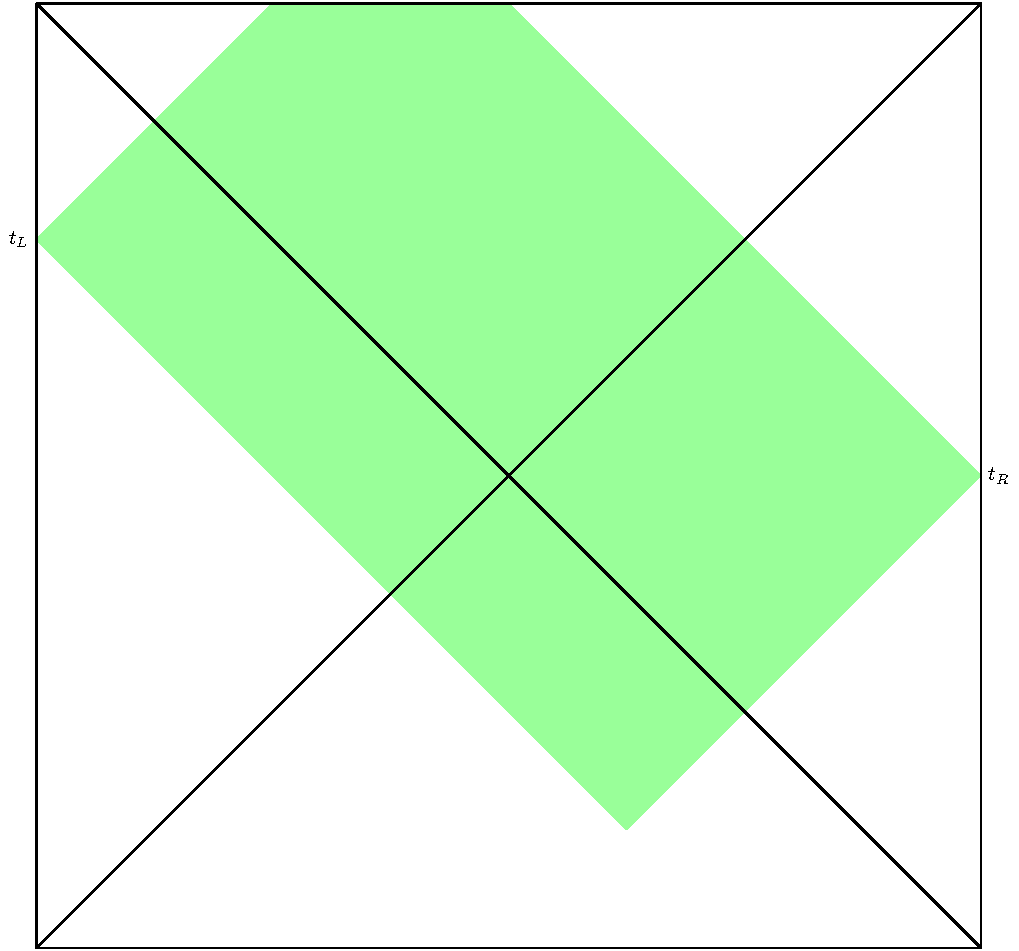
\includegraphics[scale=0.4]{WDW.pdf}    
    
    \end{center}
    \caption{The WDW patch defined by boundry times $t_L$ and $t_R$}
    \label{fig:WDW}
\end{figure}

\end{minipage}

\end{frame}


\begin{frame}
\frametitle{The WDW patch}

\begin{minipage}[t]{0.55\linewidth}

\begin{itemize}

\item The WDW patch is defined by a spatial slice of the boundary. 

\item For a two-sided black hole, this can be given by a left time $t_L$ and a right time $t_R$.

\item The WDW patch is then defined as the union of all spatial slices which meet the left boundary at $t_L$ and the right boundary at $t_R$, along with the null boundary of this region.

\item The action of this patch diverges at the boundary, so we will regularize by a cutoff

\end{itemize}

\end{minipage}\hfill
%
\begin{minipage}[t]{0.44\linewidth}

\begin{figure}
    \begin{center}
    
        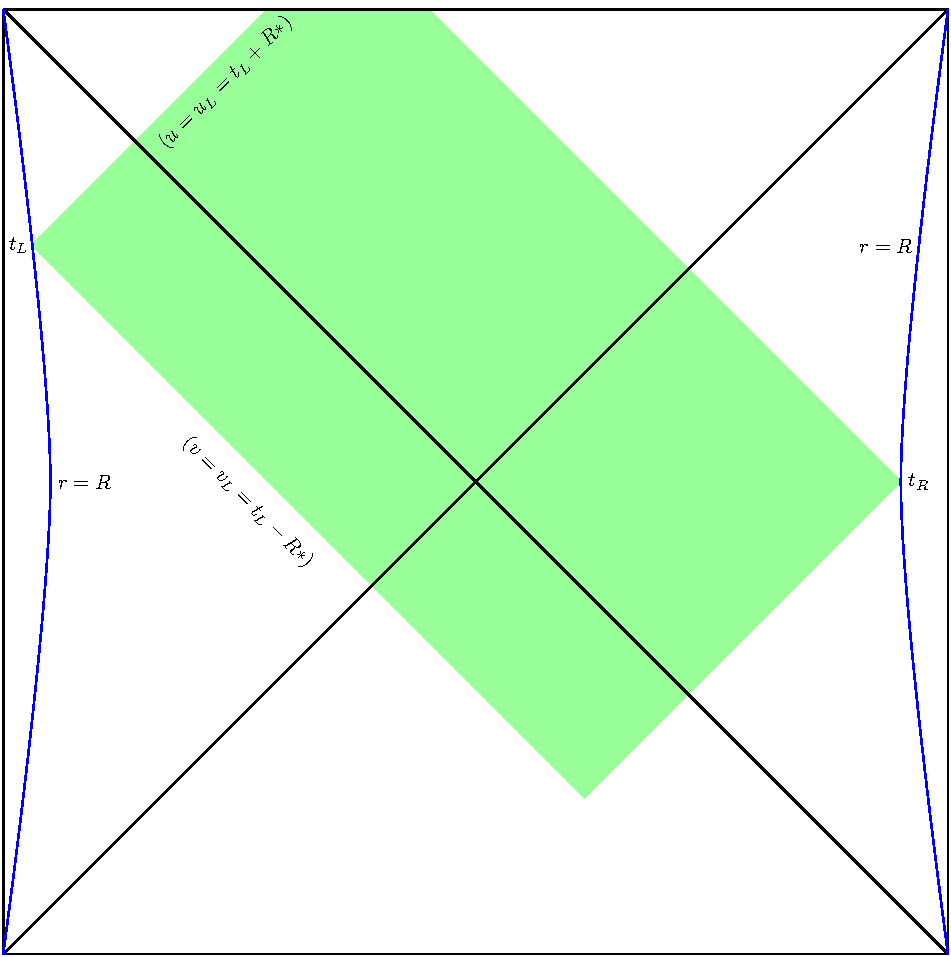
\includegraphics[scale=0.4]{WDW2.pdf}    
    
    \end{center}
    \caption{The WDW patch defined by boundry times $t_L$ and $t_R$ and a cutoff $R$}
    \label{fig:WDW2}
\end{figure}

\end{minipage}

\end{frame}


\begin{frame}
\frametitle{The WDW patch}

\begin{minipage}[t]{0.5\linewidth}

\begin{itemize}

\item The WDW patch is defined by a spatial slice of the boundary. 

\item For a two-sided black hole, this can be given by a left time $t_L$ and a right time $t_R$.

\item The WDW patch is then defined as the union of all spatial slices which meet the left boundary at $t_L$ and the right boundary at $t_R$, along with the null boundary of this region.

\item The action of this patch diverges at the boundary, so we will regularize by a cutoff

\item We will only be interested in the rate of change of the action, as $t_L$ increases.

\end{itemize}

\end{minipage}\hfill
%
\begin{minipage}[t]{0.48\linewidth}

\begin{figure}
    \begin{center}
    
        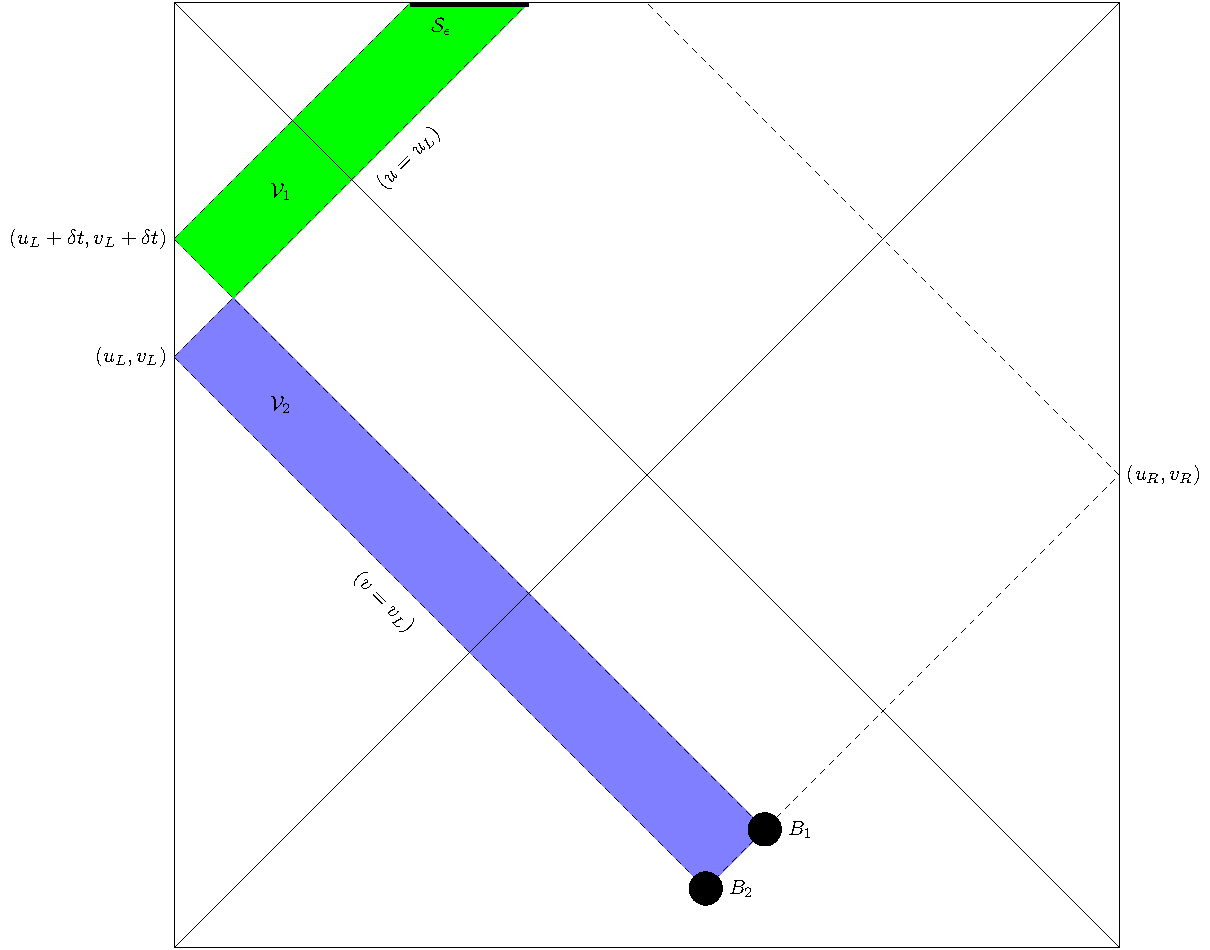
\includegraphics[scale=0.35]{2WDW.pdf}    
    
    \end{center}
    \caption{Two WDW patches separated by $\delta t$.  In thi figure, we have suppressed the cutoff}
    \label{fig:2WDW}
\end{figure}

\end{minipage}

\end{frame}


\begin{frame}
\frametitle{The WDW patch}

\begin{minipage}[t]{0.5\linewidth}

\begin{itemize}

\item The WDW patch is defined by a spatial slice of the boundary. 

\item For a two-sided black hole, this can be given by a left time $t_L$ and a right time $t_R$.

\item The WDW patch is then defined as the union of all spatial slices which meet the left boundary at $t_L$ and the right boundary at $t_R$, along with the null boundary of this region.

\item The action of this patch diverges at the boundary, so we will regularize by a cutoff

\item We will only be interested in the rate of change of the action, as $t_L$ increases.

\item This may be computed by subtracting the actions of two WDW patches, whose left time is separated by $\delta t$, and then taking the limit where $\delta t \rightarrow 0$.

\end{itemize}

\end{minipage}\hfill
%
\begin{minipage}[t]{0.48\linewidth}

\begin{figure}
    \begin{center}
    
        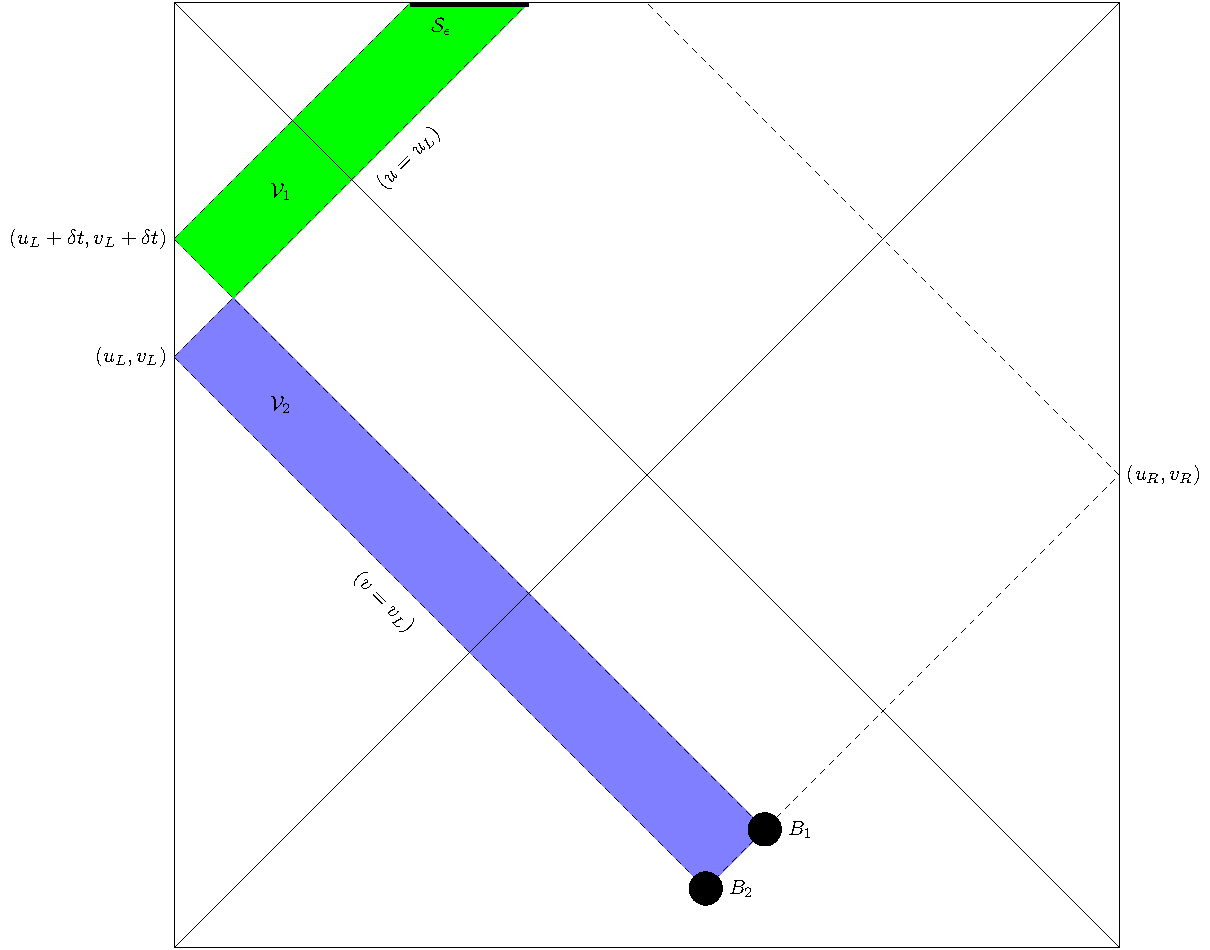
\includegraphics[scale=0.35]{2WDW.pdf}    
    
    \end{center}
    \caption{Two WDW patches separated by $\delta t$.  In thi figure, we have suppressed the cutoff}
    \label{fig:2WDW}
\end{figure}

\end{minipage}

\end{frame}


\begin{frame}
\frametitle{The WDW patch}

\begin{minipage}[t]{0.5\linewidth}

\begin{itemize}

\item The WDW patch is defined by a spatial slice of the boundary. 

\item For a two-sided black hole, this can be given by a left time $t_L$ and a right time $t_R$.

\item The WDW patch is then defined as the union of all spatial slices which meet the left boundary at $t_L$ and the right boundary at $t_R$, along with the null boundary of this region.

\item The action of this patch diverges at the boundary, so we will regularize by a cutoff

\item We will only be interested in the rate of change of the action, as $t_L$ increases.

\item This may be computed by subtracting the actions of two WDW patches, whose left time is separated by $\delta t$, and then taking the limit where $\delta t \rightarrow 0$.

\item This difference of actions decomposes to the difference of two bulk pieces, a piece from the spacelike boundary of a near singularity cutoff, and two codimension two contributions from the past corners of the patches.

\end{itemize}

\end{minipage}\hfill
%
\begin{minipage}[t]{0.48\linewidth}

\begin{figure}
    \begin{center}
    
        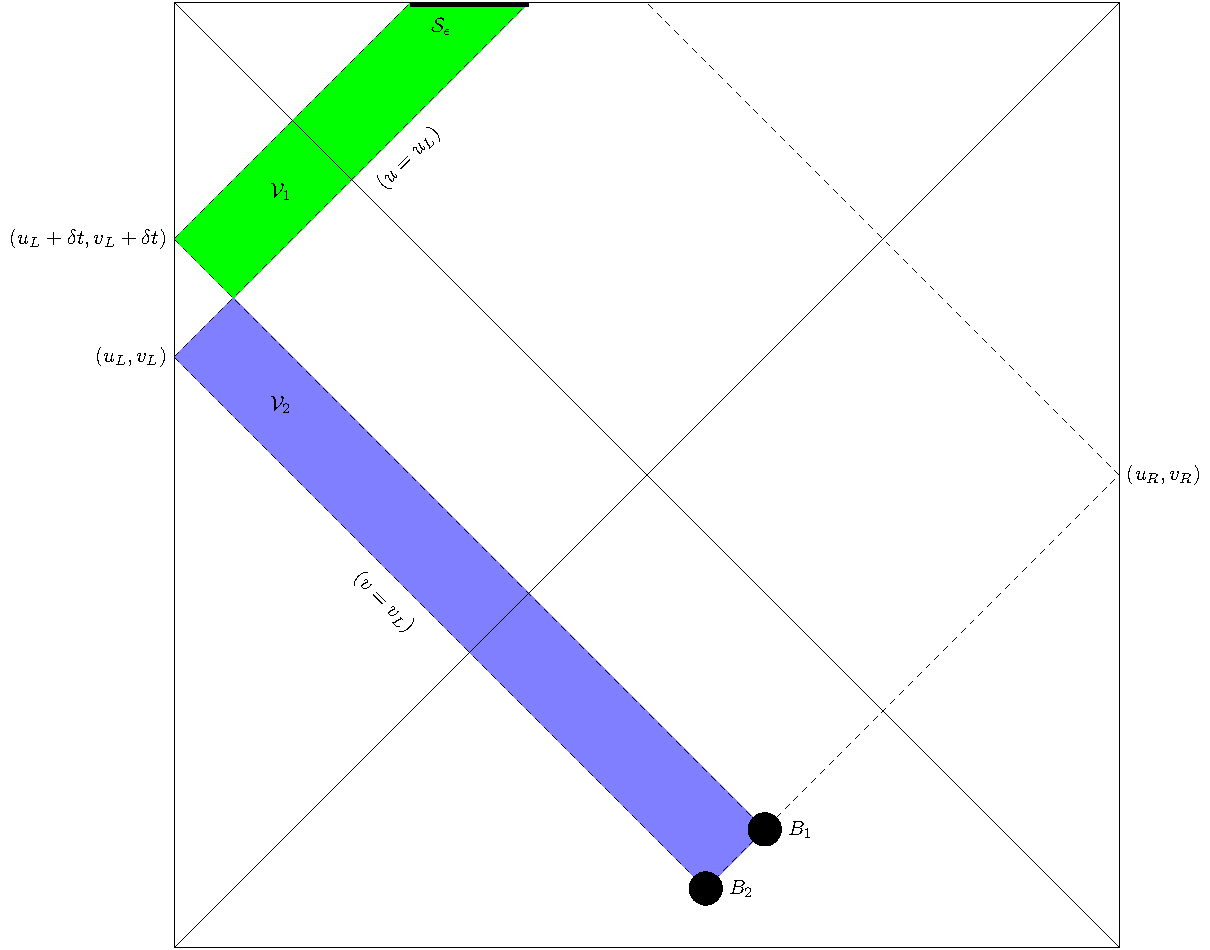
\includegraphics[scale=0.35]{2WDW.pdf}    
    
    \end{center}
    \caption{Two WDW patches separated by $\delta t$.  In thi figure, we have suppressed the cutoff}
    \label{fig:2WDW}
\end{figure}

\end{minipage}

\end{frame}


%\section{The Gravity Dual of NCSYM}

\begin{frame}
\frametitle{Why study NCSYM?}

\begin{itemize}

\item We would like to test complexity = action in a new context. 

\item Tests from strongly coupled field theory are hard, so we would like field theory with a known gravity dual

\item A gravity solution dual to NCSYM was derived in the late 90's by a number of authors \cite{Hashimoto:1999ut, Maldacena:1999mh}.

\item And this solution has been well studied in other contexts (see e.g. Cai et al. \cite{Cai:1999aw}, Edlati et al. \cite{Edalati:2012jj}, Fischler et al. \cite{Fischler:2013gsa}, Karczmarek et al. \cite{Karczmarek:2013xxa}).

\item Also, generalizations of this system to other numbers of dimensions have also been considered in, e.g., Alishahiha et al. \cite{Alishahiha:1999ci} and Berman et al. \cite{Berman:2000jw}.

\item These theories come with a tunable parameter in the Moyal scale, so that the behavior of complexity with this parameter may be studied

\end{itemize}

\end{frame}

\begin{frame}
\frametitle{The gravity dual to NCSYM}

The gravity dual to NCSYM is obtained in a manner similar to that of standard $\mathcal{N} = 4$ SYM.

\begin{itemize}

\item Consider a stack of D3-branes

\item We turn on a 2-form B parallel to the two spatial dimensions of the branes

\item This can be achieved by applying a combination of T-dualities and Gauge transformations

\item The B-field has the effect of introducing non-commutativity in the worldbrane theory

\item The near horizon geometry in the usual limit gives the gravity dual, which is a IIB SUGRA solution.

\end{itemize}

The resulting solution, at finite teperature, is given in Einstein frame as follows:

\begin{equation}
ds^2 = \alpha' \bigg[ \left(\frac{r}{L}\right)^2
\left(- f(r) dt^2 + dx_1^2  + h(r) (dx_2^2 + dx_3^2)\right)
+\left(\frac{L}{r}\right)^2 \left(
\frac{dr^2}{f(r)} + r^2 d\Omega_5^2\right)\bigg],
\end{equation}
%
\begin{equation}
e^{2\Phi} = \hat{g}_s^2 h(r) ,\quad B_{23} = B_{\infty}(1-h(r)) ,\quad C_{01} = -\frac{\alpha^{\prime} a^2 r^4}{\hat{g}_s R^2} ,\quad F_{0123r} = \frac{4\alpha^{\prime 2} r^3}{\hat{g}_s R^4} h(r)
\end{equation}
%
\begin{equation}
f(r) = 1 - \left(\frac{r_+}{r}\right)^4 ,\quad h(r) = \frac{1}{1 + a^4 r^4} ,\quad B_{\infty} = -\frac{\alpha'}{a^2 L^2}. 
\end{equation}

Here $L$ is the AdS length scale, $r_+$ is the bulk coordinate of the horizon, $\hat{g}_s$ is the  and closed string coupling, and $a$ is the Moyal scale (i.e. $[x_2,x_3]= i a^2$ on the boundary).

\end{frame}

\begin{frame}
\frametitle{The gravity dual to NCSYM}

A few additional notes about the gravity dual:

\begin{itemize}

\item The bulk coordinate $r$ has units of inverse length.

\item Though the boundary field theory lives on a non-commutative manifold, the bulk geometry is commutative.

\item The metric degenerates at the boundary. This should be fine, however, provided we always work with a finite cutoff.

\item The dimension of the Hilbert space in the dual theory was found to be independent of the Moyal scale by Maldacena and Russo in \cite{Maldacena:1999mh}.

\end{itemize}

We will now consider an intuition based heuristic argument that we should expect the complexity at a given (late) time should be higher in NCSYM than in it's commutative counterpart.

\end{frame}

\begin{frame}
\frametitle{Non-Commutativity and Complexity: A heuristic argument}

\begin{minipage}[t]{0.5\linewidth}

\begin{itemize}

\item Consider the unitary operator $U$ which translates our state in time by a small time $\delta t$. 

\end{itemize}

\end{minipage}\hfill
%
\begin{minipage}[t]{0.48\linewidth}

\begin{figure}
    \begin{center}
    
        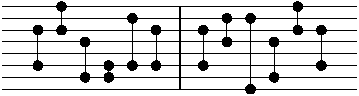
\includegraphics[scale=1]{animation/animation_1}    
        
        \vspace{2mm}
        
        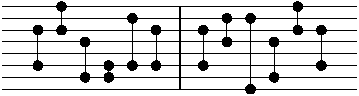
\includegraphics[scale=1]{animation/animation_1}    
    
    \end{center}
    \caption{A small piece of a circuit implementing time translations on a local (top) and non-local (bottom) theory. This cartoon is inspired by another which appears in certain talks by Adam Brown.}
\end{figure}

\end{minipage}

\end{frame}


\begin{frame}
\frametitle{Non-Commutativity and Complexity: A heuristic argument}

\begin{minipage}[t]{0.5\linewidth}

\begin{itemize}

\item Consider the unitary operator $U$ which translates our state in time by a small time $\delta t$. 

\item Consider further an optimal circuit $Q$ implementing $U$.

\end{itemize}

\end{minipage}\hfill
%
\begin{minipage}[t]{0.48\linewidth}

\begin{figure}
    \begin{center}
    
        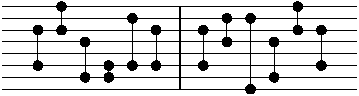
\includegraphics[scale=1]{animation/animation_1}    
        
        \vspace{2mm}
        
        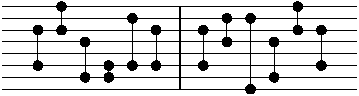
\includegraphics[scale=1]{animation/animation_1}    
    
    \end{center}
    \caption{A small piece of a circuit implementing time translations on a local (top) and non-local (bottom) theory. This cartoon is inspired by another which appears in certain talks by Adam Brown.}
\end{figure}

\end{minipage}

\end{frame}


\begin{frame}
\frametitle{Non-Commutativity and Complexity: A heuristic argument}

\begin{minipage}[t]{0.5\linewidth}

\begin{itemize}

\item Consider the unitary operator $U$ which translates our state in time by a small time $\delta t$. 

\item Consider further an optimal circuit $Q$ implementing $U$.

\item At late time $t$, the circuit $Q^N$ approximates $U^N$, where $N= t/\delta t$.

\end{itemize}

\end{minipage}\hfill
%
\begin{minipage}[t]{0.48\linewidth}

\begin{figure}
    \begin{center}
    
        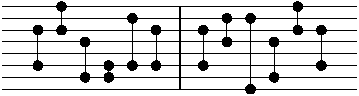
\includegraphics[scale=1]{animation/animation_1}    
        
        \vspace{2mm}
        
        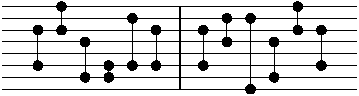
\includegraphics[scale=1]{animation/animation_1}    
    
    \end{center}
    \caption{A small piece of a circuit implementing time translations on a local (top) and non-local (bottom) theory. This cartoon is inspired by another which appears in certain talks by Adam Brown.}
\end{figure}

\end{minipage}

\end{frame}


\begin{frame}
\frametitle{Non-Commutativity and Complexity: A heuristic argument}

\begin{minipage}[t]{0.5\linewidth}

\begin{itemize}

\item Consider the unitary operator $U$ which translates our state in time by a small time $\delta t$. 

\item Consider further an optimal circuit $Q$ implementing $U$.

\item At late time $t$, the circuit $Q^N$ approximates $U^N$, where $N= t/\delta t$.

\item This circuit is generally non-optimal however, as there will be gates which cancel between the beginning and end of successive copies of $Q$.

\end{itemize}

\end{minipage}\hfill
%
\begin{minipage}[t]{0.48\linewidth}

\begin{figure}
    \begin{center}
    
        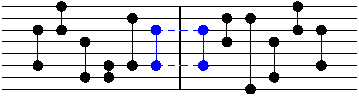
\includegraphics[scale=1]{animation/animation_2}    
        
        \vspace{2mm}
        
        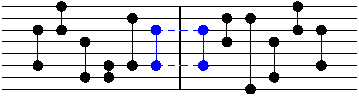
\includegraphics[scale=1]{animation/animation_2}    
    
    \end{center}
    \caption{A small piece of a circuit implementing time translations on a local (top) and non-local (bottom) theory. This cartoon is inspired by another which appears in certain talks by Adam Brown.}
\end{figure}

\end{minipage}

\end{frame}


\begin{frame}
\frametitle{Non-Commutativity and Complexity: A heuristic argument}

\begin{minipage}[t]{0.5\linewidth}

\begin{itemize}

\item Consider the unitary operator $U$ which translates our state in time by a small time $\delta t$. 

\item Consider further an optimal circuit $Q$ implementing $U$.

\item At late time $t$, the circuit $Q^N$ approximates $U^N$, where $N= t/\delta t$.

\item This circuit is generally non-optimal however, as there will be gates which cancel between the beginning and end of successive copies of $Q$.

\item These cancelations lead to a circuit for the same operator of lower complexity

\end{itemize}

\end{minipage}\hfill
%
\begin{minipage}[t]{0.48\linewidth}

\begin{figure}
    \begin{center}
    
        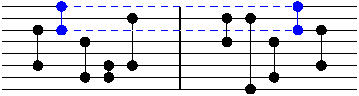
\includegraphics[scale=1]{animation/animation_3}    
        
        \vspace{2mm}
        
        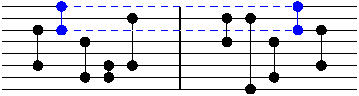
\includegraphics[scale=1]{animation/animation_3}    
    
    \end{center}
    \caption{A small piece of a circuit implementing time translations on a local (top) and non-local (bottom) theory. This cartoon is inspired by another which appears in certain talks by Adam Brown.}
\end{figure}

\end{minipage}

\end{frame}


\begin{frame}
\frametitle{Non-Commutativity and Complexity: A heuristic argument}

\begin{minipage}[t]{0.5\linewidth}

\begin{itemize}

\item Consider the unitary operator $U$ which translates our state in time by a small time $\delta t$. 

\item Consider further an optimal circuit $Q$ implementing $U$.

\item At late time $t$, the circuit $Q^N$ approximates $U^N$, where $N= t/\delta t$.

\item This circuit is generally non-optimal however, as there will be gates which cancel between the beginning and end of successive copies of $Q$.

\item These cancelations lead to a circuit for the same operator of lower complexity

\item In a non-local theory (such as a non-commutative theory), fewer operators commute past one another, and so there will be more obstruction to such cancelations, leading to a higher final complexity.

\end{itemize}

\end{minipage}\hfill
%
\begin{minipage}[t]{0.48\linewidth}

\begin{figure}
    \begin{center}
    
        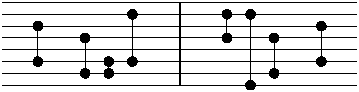
\includegraphics[scale=1]{animation/animation_4}    
        
        \vspace{2mm}
        
        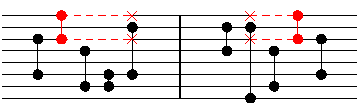
\includegraphics[scale=1]{animation/animation_5}    
    
    \end{center}
    \caption{A small piece of a circuit implementing time translations on a local (top) and non-local (bottom) theory. This cartoon is inspired by another which appears in certain talks by Adam Brown.}
\end{figure}

\end{minipage}

\end{frame}

%\section{Results}

\begin{frame}
\frametitle{Results}

Now that we have this na\"ive expectation, we will compare with the complexity in NCSYM according to CA. We will find it convenient to define the parameters $b = a r_+ = \pi a T$,  $\rho = \frac{r_B}{r_+}$, and  $\gamma = \frac{c \bar{c} \sqrt{\bar{g}_s} L^2}{\alpha' \pi^2 T^2}$.
\begin{itemize}

\item $T=\pi r_+$ is the temperature

\item $c$ and $\bar{c}$ are the normalizations of the null generators

\end{itemize}

With these conventions, the complexification rate after the critical time is given by

\begin{equation}
\dot{C} = \frac{\Omega_5 V_3 r_+^4}{(2\pi)^7 \hat{g}_s^2}
\bigg(\frac{-2\log(1+b^4 \rho^4)}{b^4}+4\rho^4+6+3(1-\rho^4)\log\big|\frac{\gamma \rho^2}{(1+b^4 \rho^4)^{1/4}(1-\rho^4)}\big|\bigg).
\end{equation}

Here $V_3$ is the volume of a spatial slice of the boundary theory (which is infinite) and $\Omega_3$ is the volume of a unit 5-sphere. In what follows, we will normalize the rates by the $b=0$ result. 

\end{frame}

\begin{frame}
\frametitle{D3-brane results: Finite time behavior}

In the commutative limit, we see similar behavior to that reported by Carmi et al. \cite{Carmi:2017jqz}.

\begin{minipage}[t]{0.48\linewidth}

\begin{itemize}

\item Logarithmic divergence at the critical time.

\item Reaches true global maximum in order one time (in thermal units).

\item approaches asymptotic value from above.

\end{itemize}

This behavior persists for all values of the Moyal scale  but as the Moyal scale becomes very large, the true maximum shrinks and the asymptotic value increases, so that the gap between them decreases

\end{minipage}
%
\begin{minipage}[t]{0.48\linewidth}

\begin{figure}
    \begin{center}
        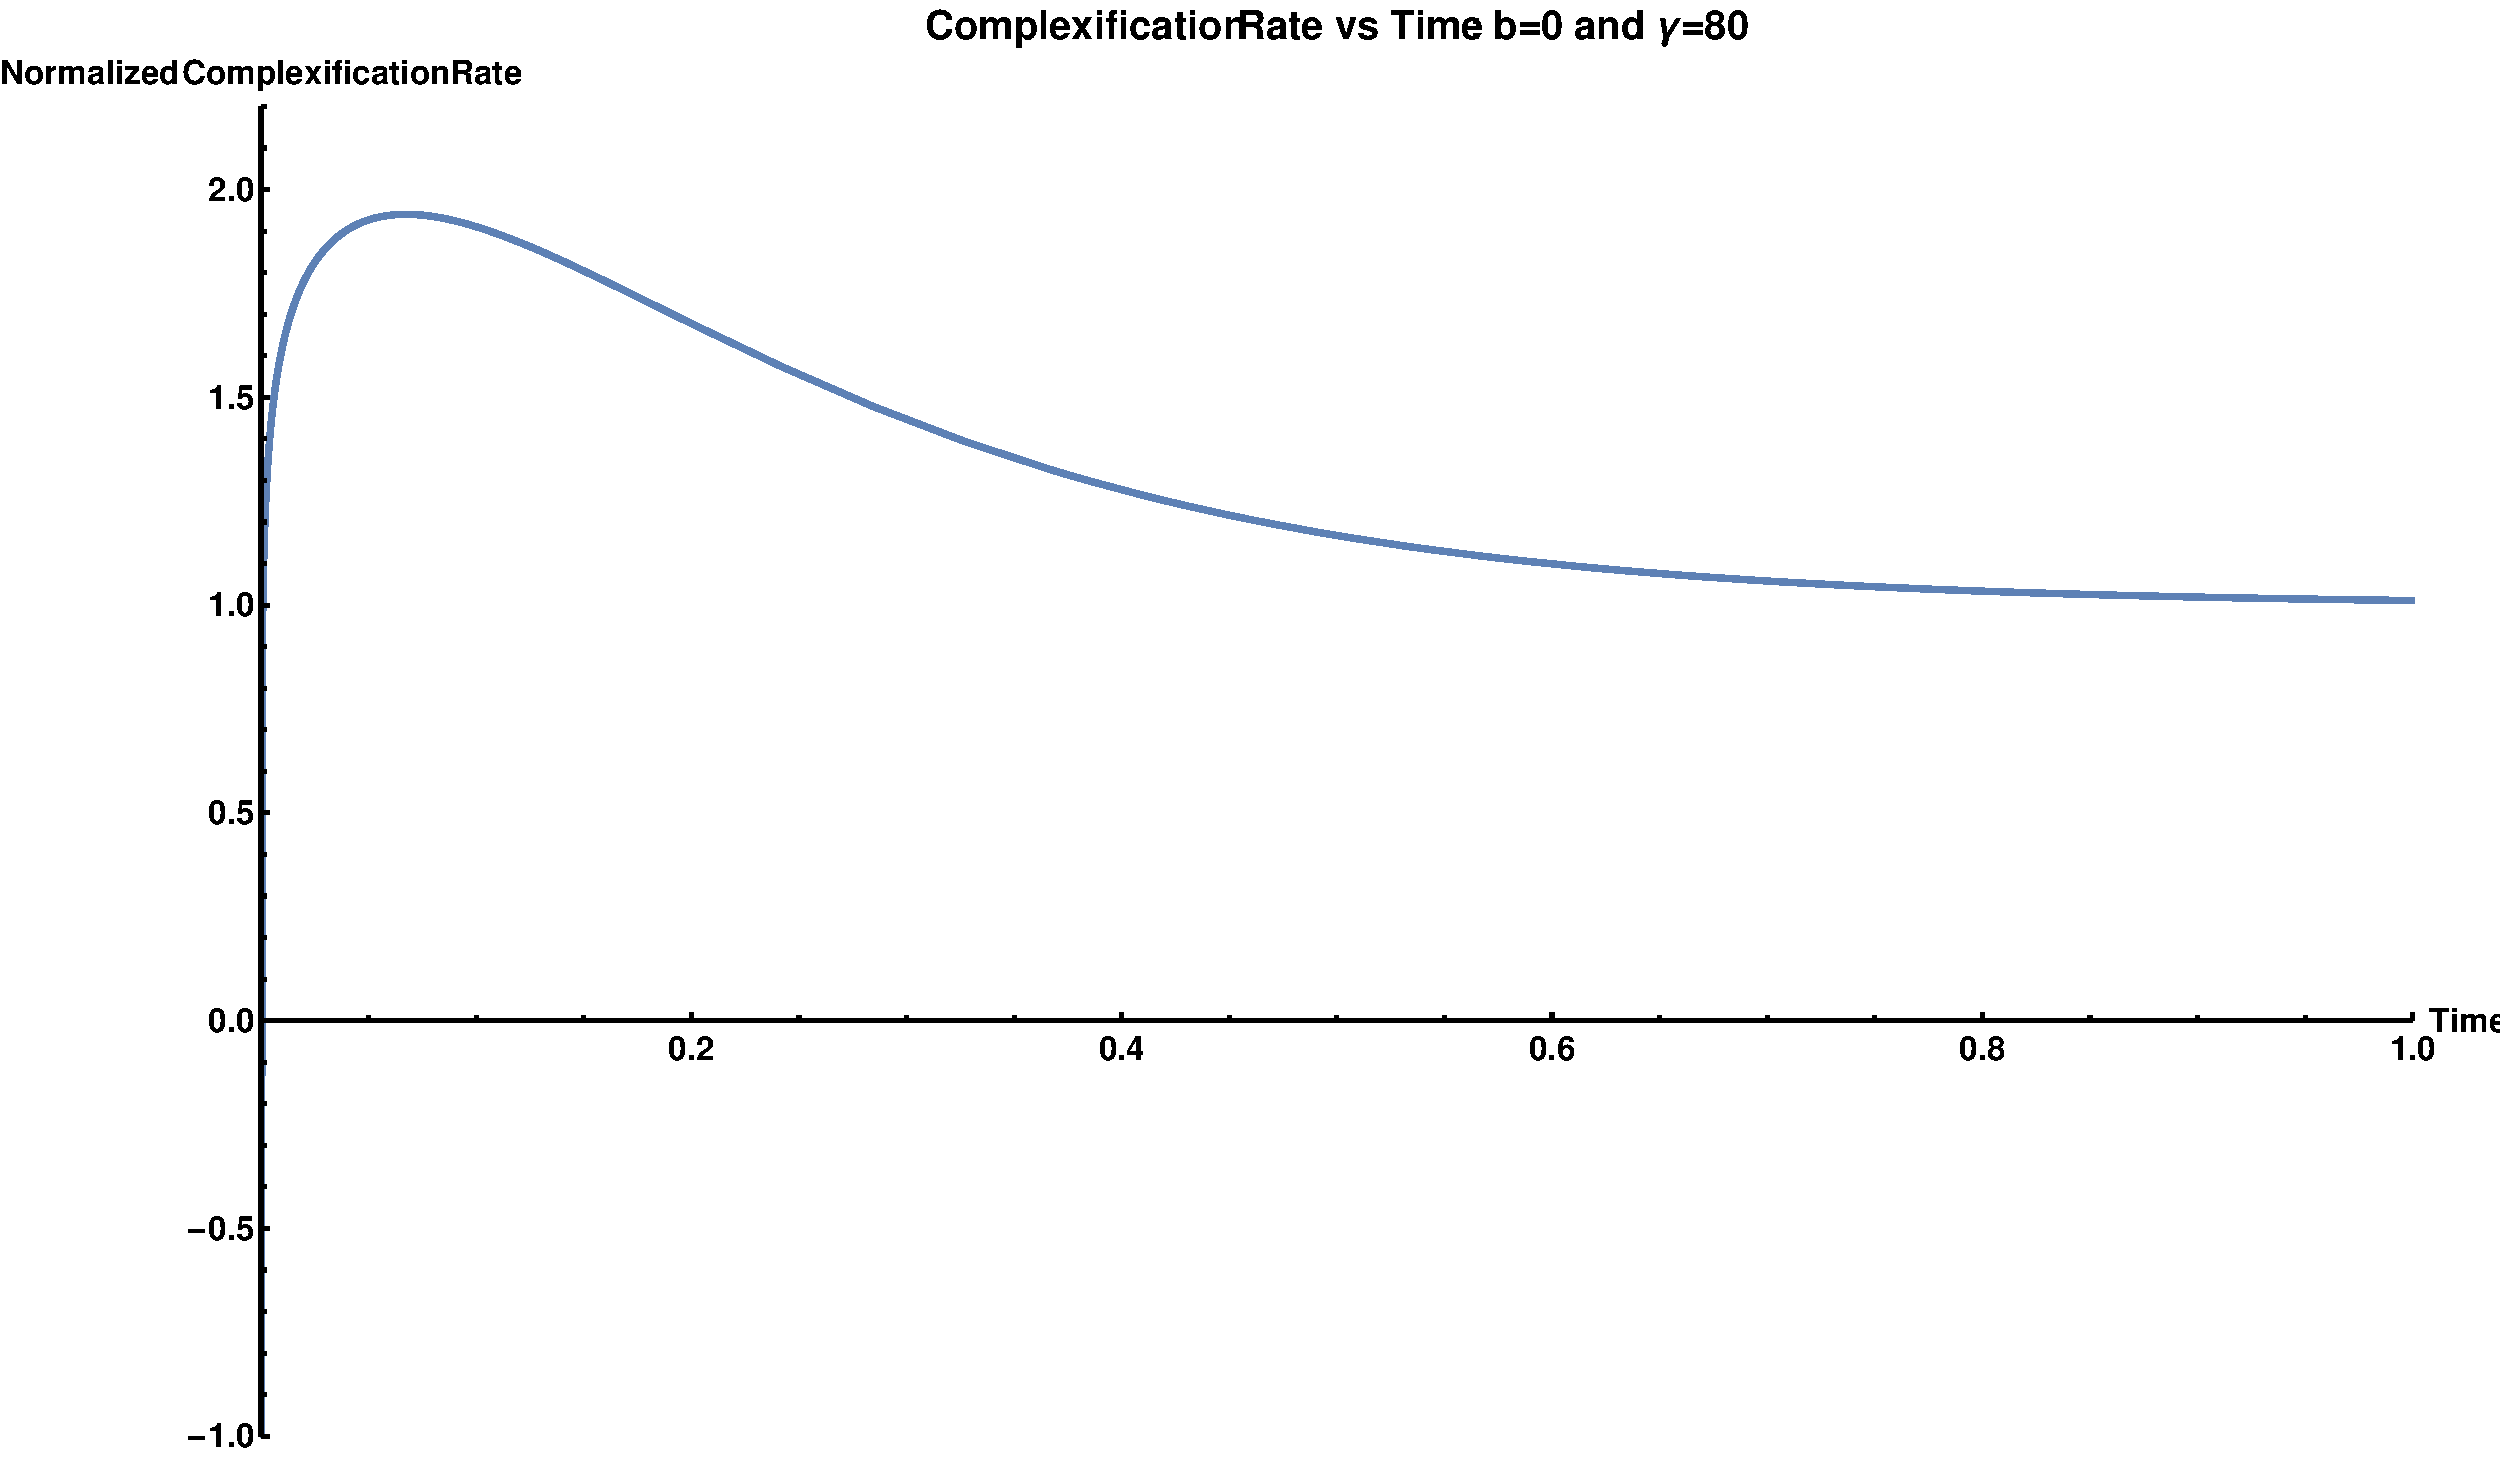
\includegraphics[scale=0.15]{FiniteTime1}
    \end{center}
\end{figure}

\end{minipage}
\vspace{5mm}

This behavior calls into question the normalization to complexity = action as set by Brown et al. \cite{Brown:2015bva, Brown:2015lvg}, though the logic that to that normalization would seem already to be contradicted by Cottrell and Montero \cite{Cottrell:2017ayj}.

\end{frame}

\begin{frame}
\frametitle{Finite time behavior}

Here we see how the finite time behavior changes as we vary the parameters.

\begin{minipage}[t]{0.47\linewidth}

\begin{figure}
    \begin{center}
        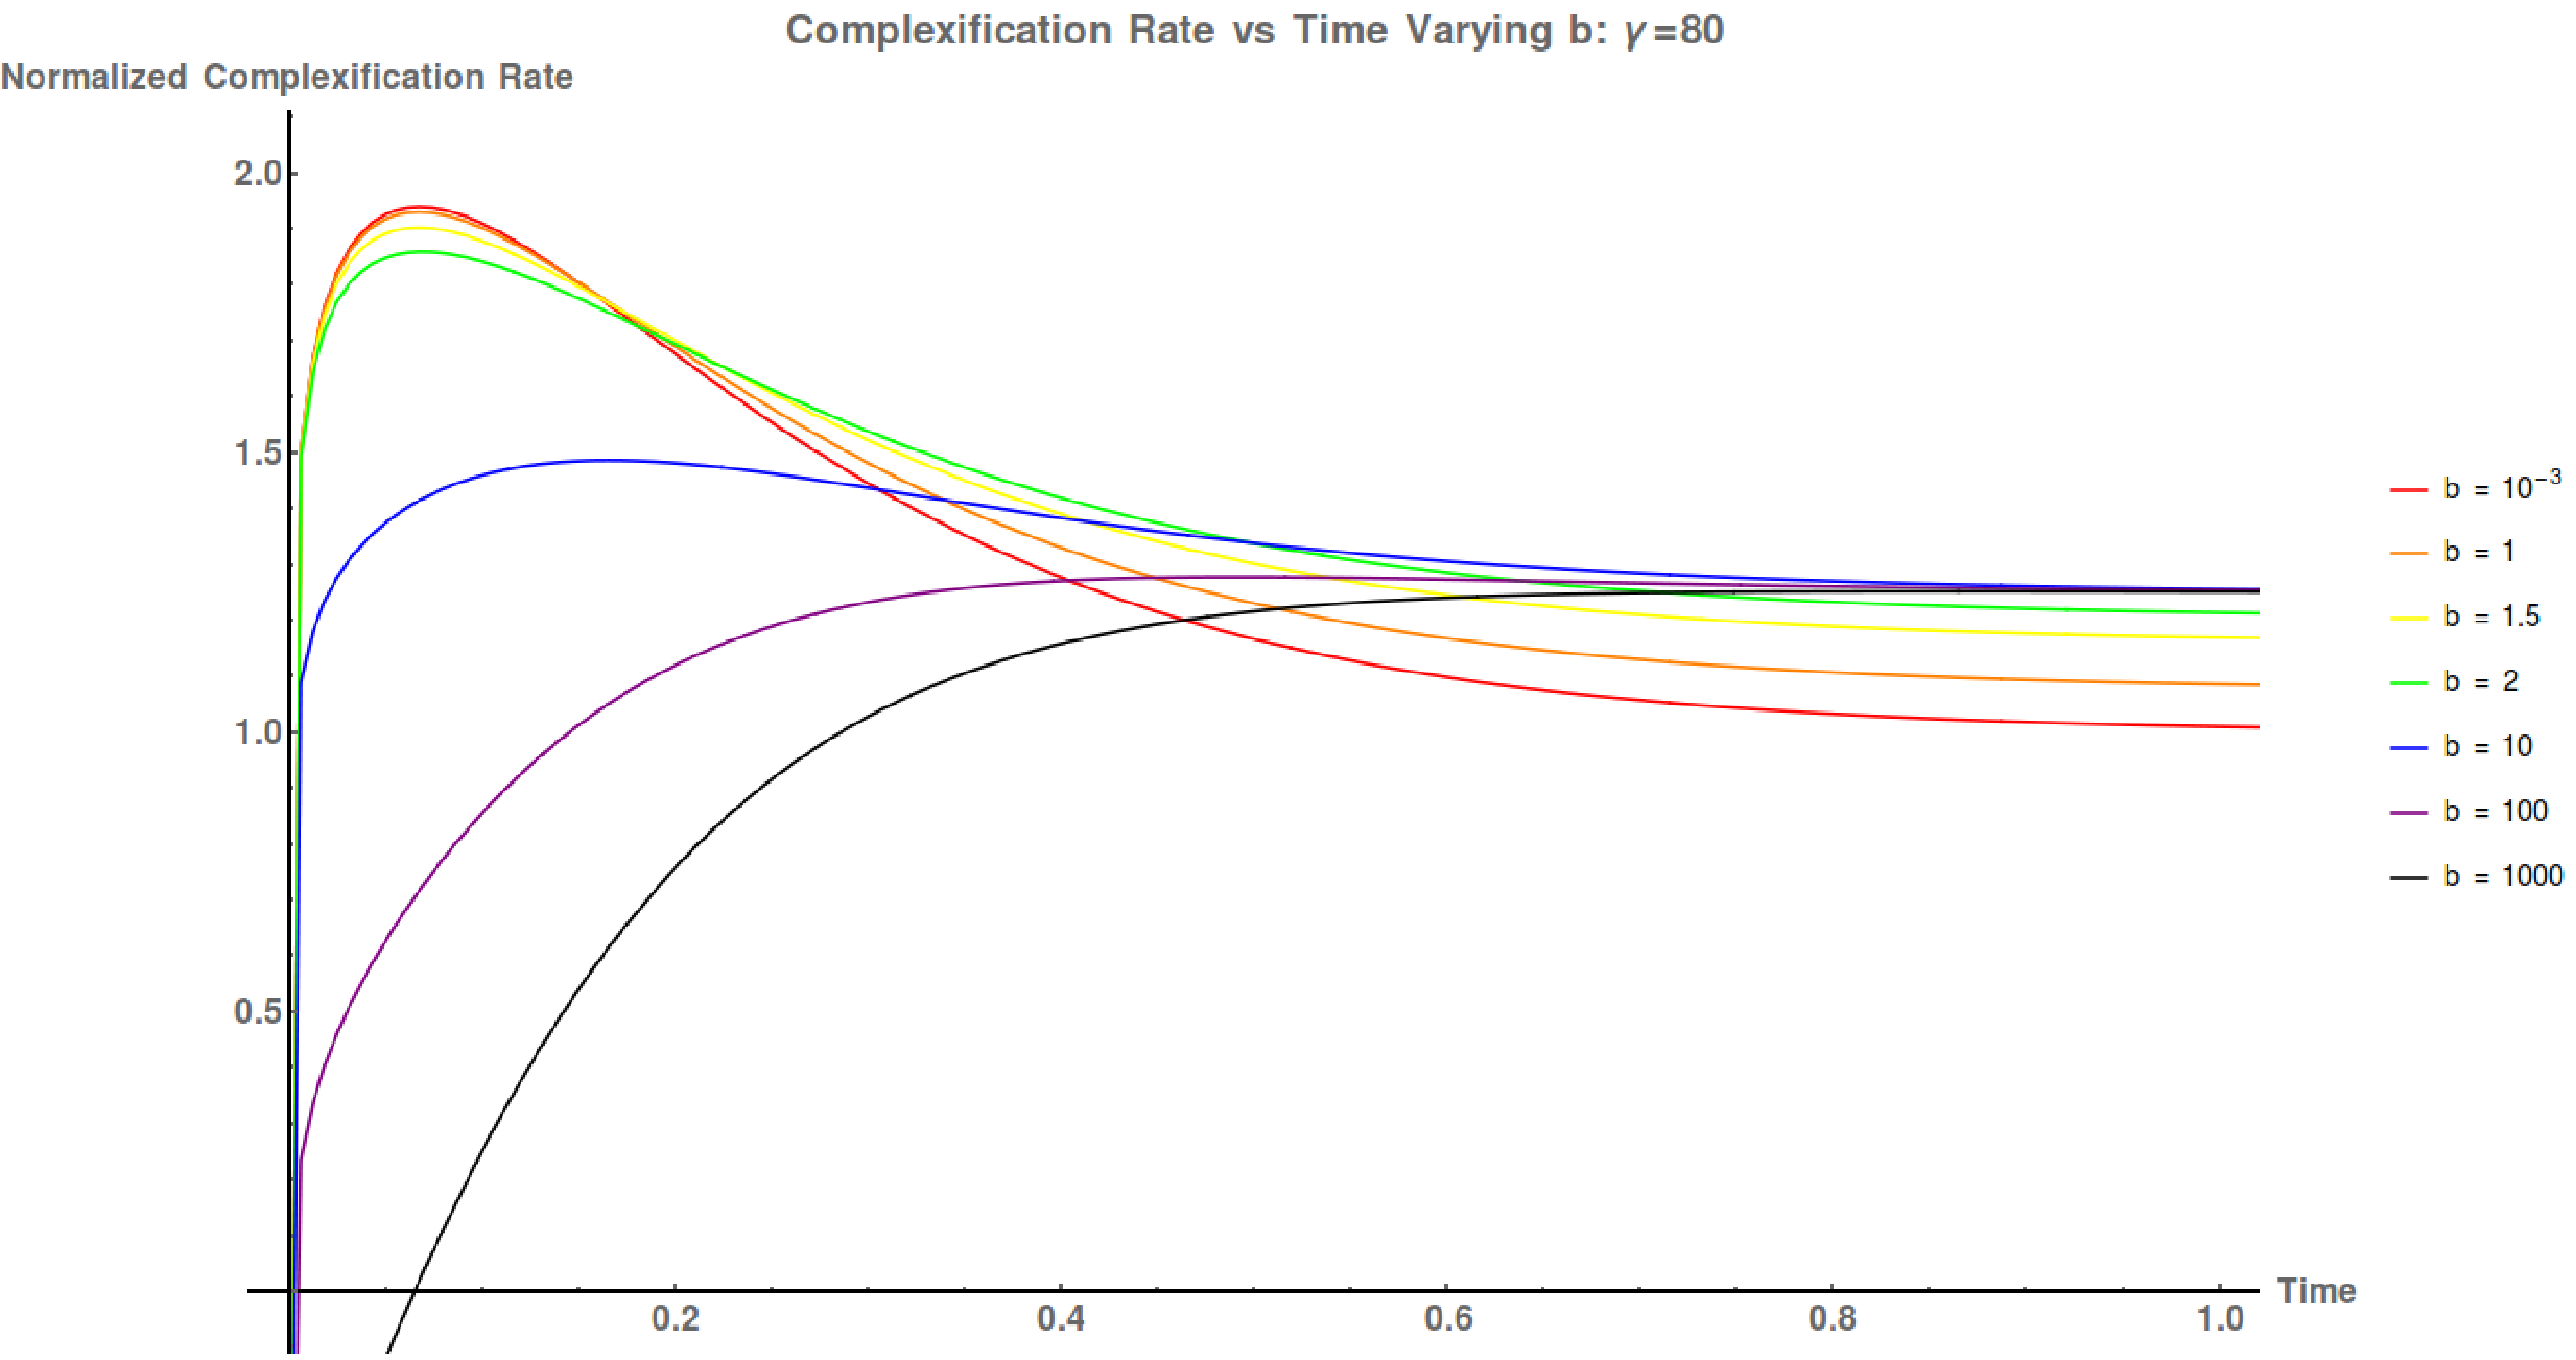
\includegraphics[scale=0.15]{vary_b_fix_gamma}
    \end{center}
\end{figure}

\end{minipage}\hfill
%
\begin{minipage}[t]{0.47\linewidth}

\begin{figure}
    \begin{center}
        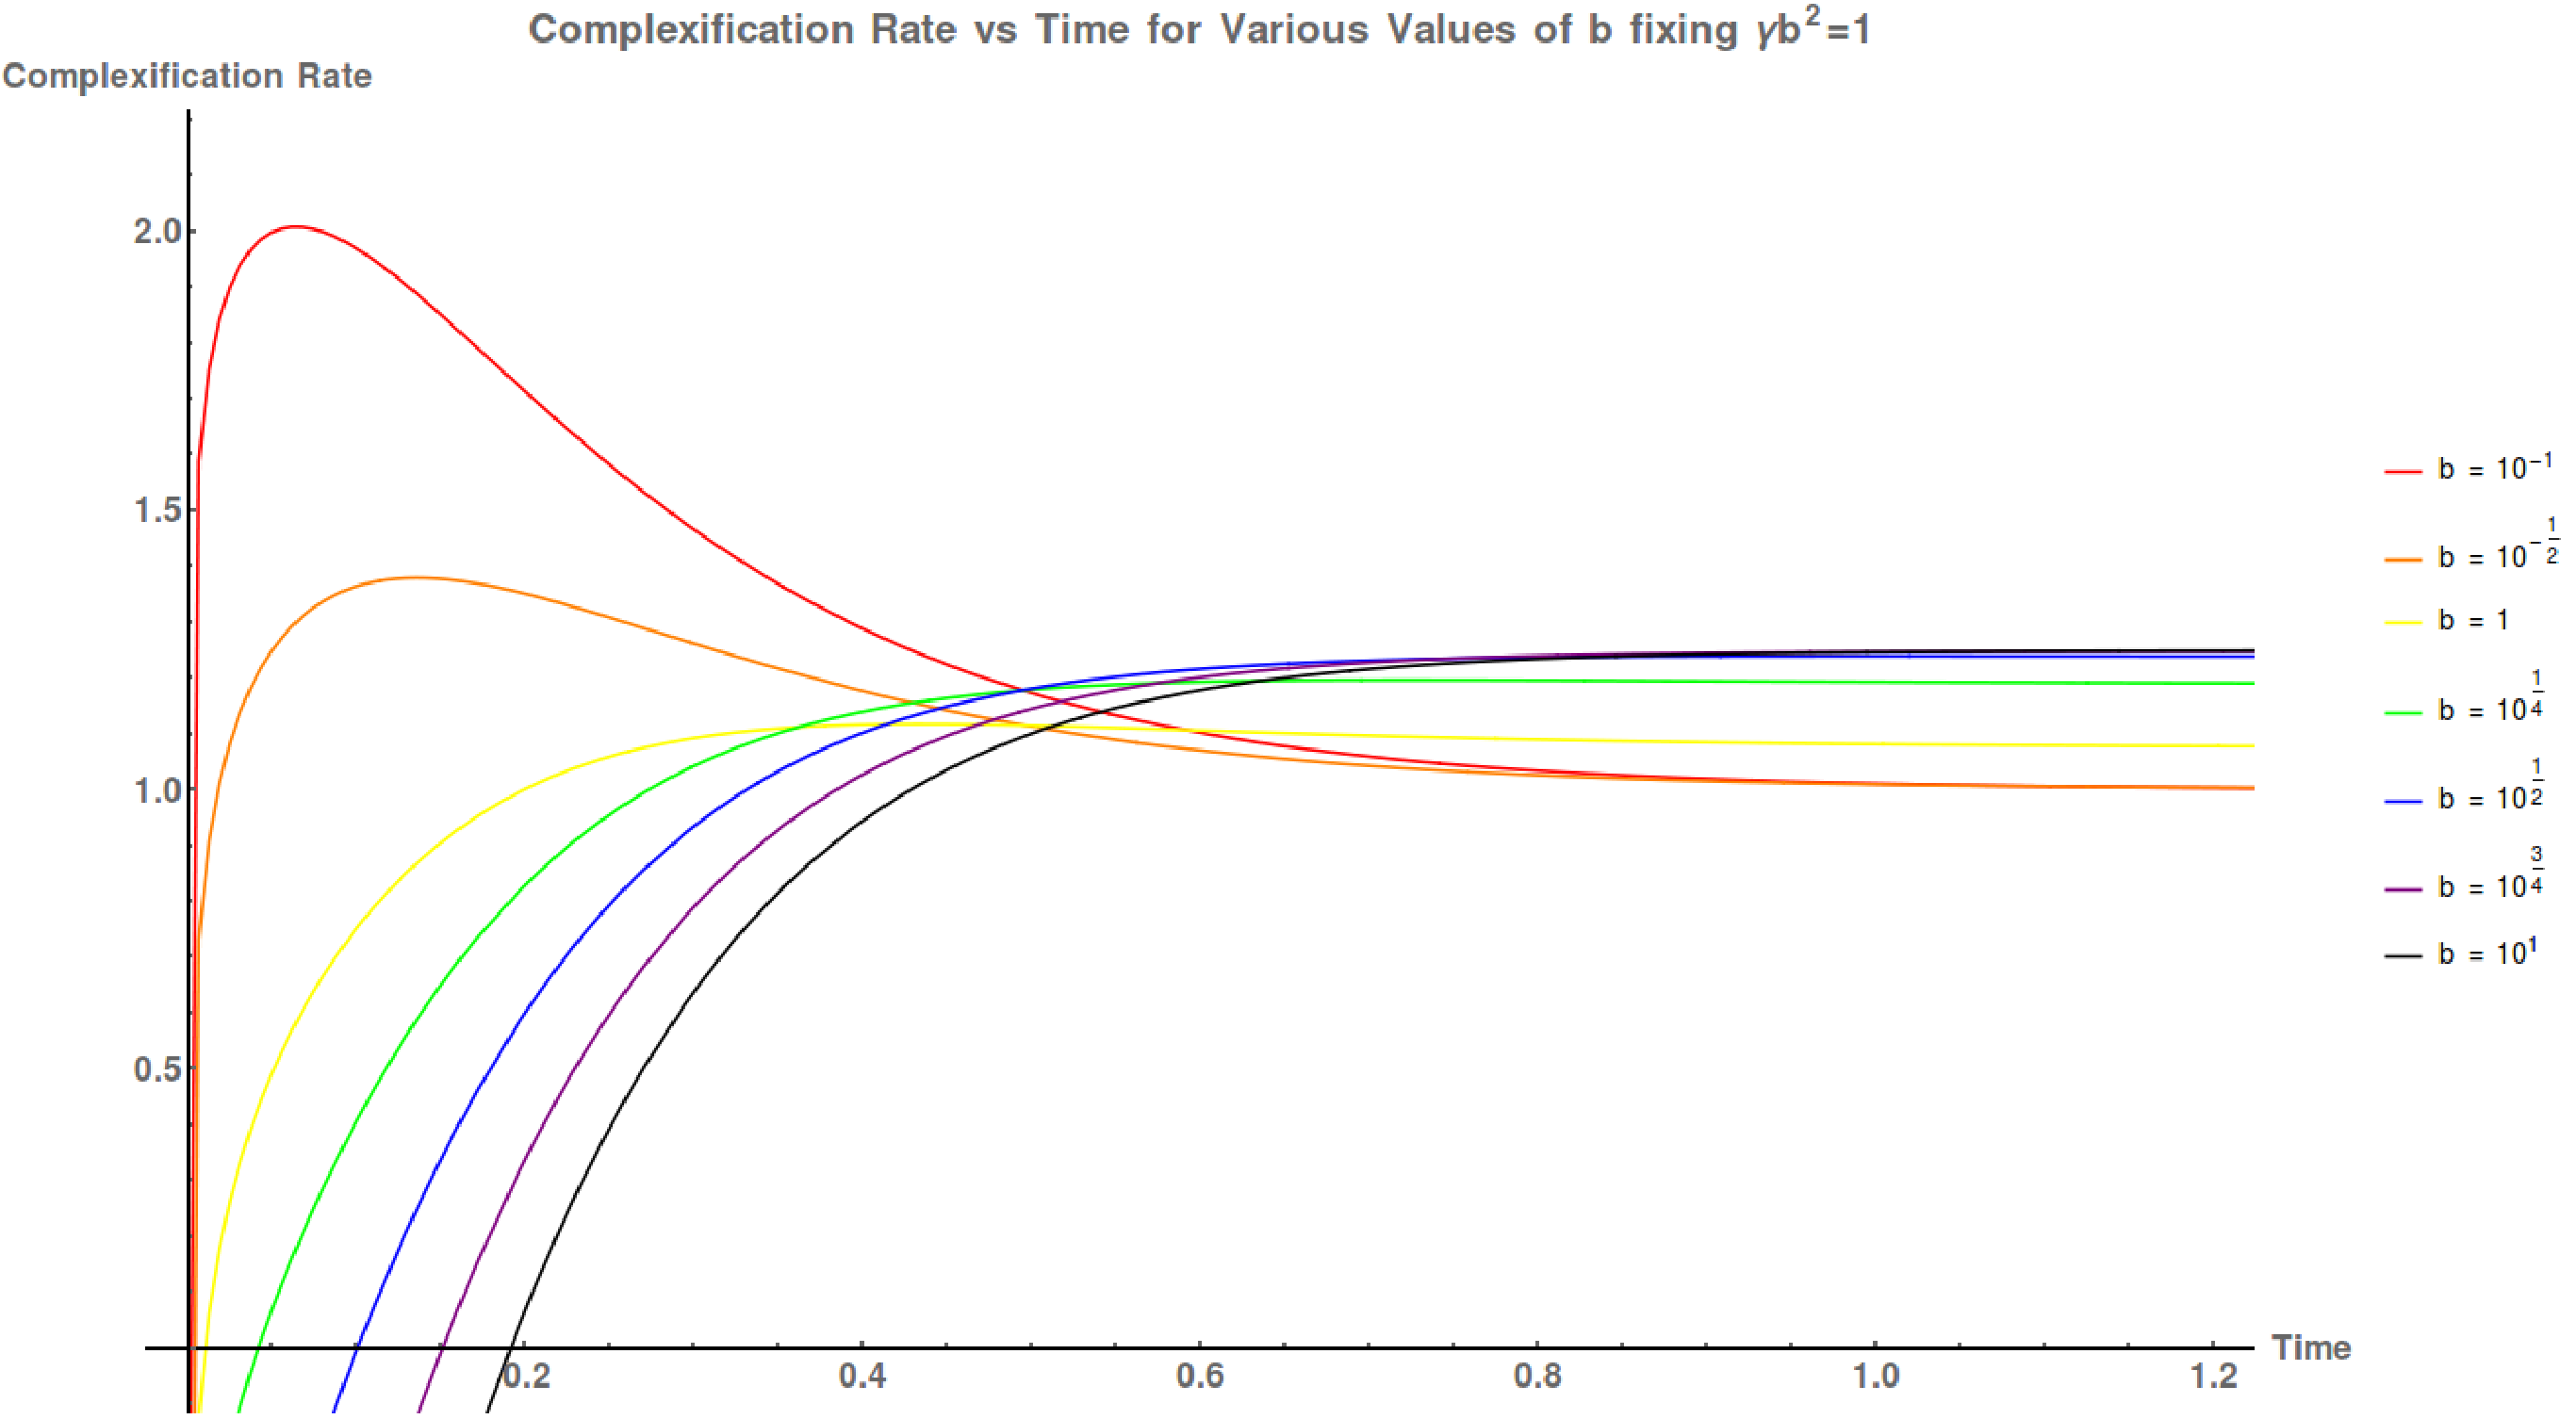
\includegraphics[scale=0.15]{vary_temp}
    \end{center}
\end{figure}

\end{minipage} 

\end{frame}

\begin{frame}
\frametitle{D3-brane results: Late time limit}

We take the late time limit by sending $r_b$ to $r_+$ (i.e. we send $\rho$ to 1). In this limit, the normalized complexification rate becomes

\begin{equation}
\dot{C}_{\text{normalized}} \large|_{t\rightarrow \infty} = \frac{5}{4}-\frac{\log(1+b^4)}{4 b^4}.
\end{equation}

Recalling that $b = \pi a T$, we see that at a fixed temperature, as we send the Moyal scale to infinity, we get $5/4$, which given the normalization scheme tells us that we get exactly a 25\% enhancement in of the complexification rate in the large Moyal scale regime.

\begin{figure}[htbp]
    \begin{center}
        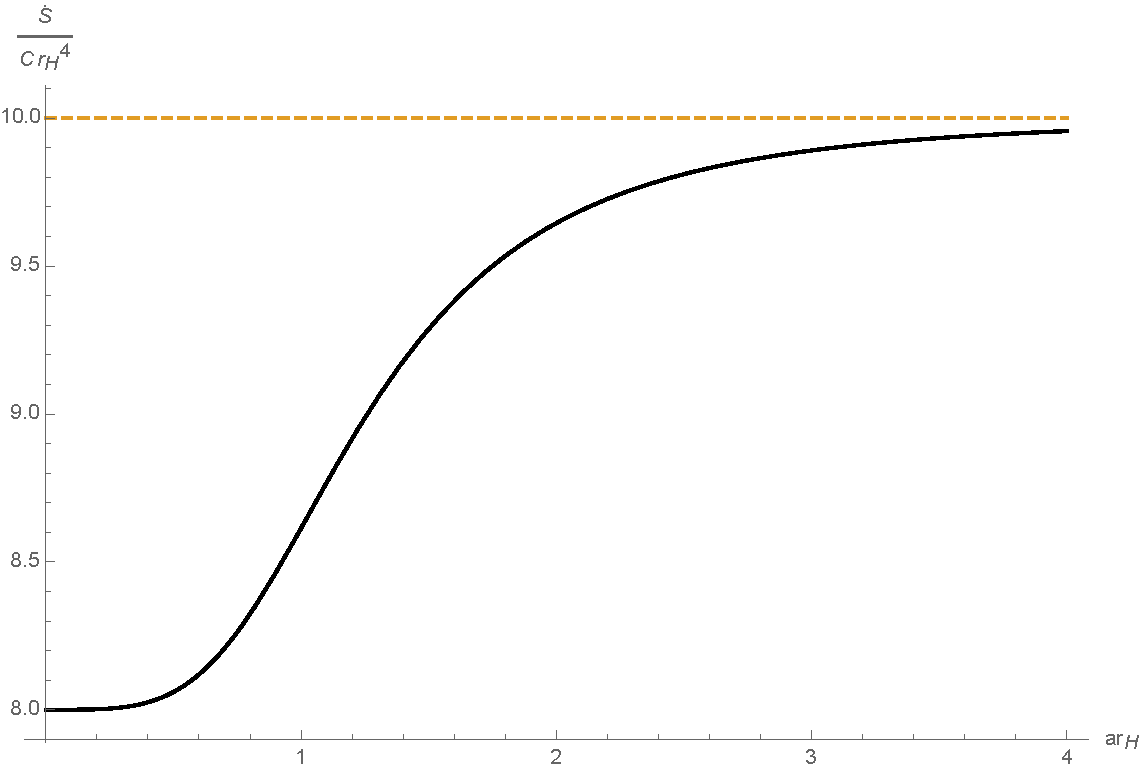
\includegraphics[scale=0.3]{LateTime}
    \end{center}
    \caption{Late time action growth rate normalized by $C=\frac{\alpha^4 \Omega_5 V_3}{\hat{g}_s^2}$ and extra $r_H$ dependence, versus $a r_+$, which is the Moyal scale measured in units of thermal length.} 
    \label{fig:LateTime}
\end{figure}

\end{frame}

\begin{frame}
\frametitle{Results for other values of $p$}

As discussed before, the geometry we have considered so far can be generalized by starting with stacks of $Dp-branes$ with for other values of $p$. For $p\neq 3$, the resulting geometry is not asymptotically AdS, even in the commutative limit. We considered $2\leq p \leq 5$. For $p\geq 4$ there is the possibility of introducing non-commutativity between multiple pairs of coordinates. The table below summarizes our results for the late time rate of change of the complexity density, with a common normalization for all results. Here $m$ indicates the number of pairs of non-commuting coordinates on the boundary.   

\begin{table}
    \centering
    \begin{tabular}{l | c  c  c }
        $p$ & $m=0$ & $m=1$ & $m=2$ \\
        \hline
        2 & 12 & 12 & - \\
        3 & 8 & 10 & - \\
        4 & 5 & 5 & 8 \\
        5 & 4 & 5 & 6 \\
    \end{tabular}
\end{table}

\end{frame}

\begin{frame}
\frametitle{Conclusions}

\begin{itemize}

\item For $p=3,5$ we do see an increase at late time, as expected.

\item Though we did not see an increase for $p=2$ or for $p=4$ with a single non-trivial commutator, at least we did not see a decrease either.

\item Overall, the results are consistent with the heuristic argument above.

\item This result is in tension with the idea that commutative black holes are the fastest possible computers

\item In future work, we plan to repeat our calculations for complexity = volume.

\end{itemize}

\end{frame}

\begin{frame}
\frametitle{References}
{\tiny
\bibliographystyle{JHEP} %JHEP.bst
\footnotesize\bibliography{NCG} %NCG.bib
}
\end{frame}

%\section{Backup Slides}

%\begin{frame}
%\frametitle{Holographic Complexity}

%\begin{itemize}

%\item Consider a two-sided black hole in asymptotically AdS space.

%\item A holographic puzzle: what could be dual to the geometry behind the horizon?

%    \begin{itemize}
    
%    \item AdS/CFT $\Rightarrow$ a two-sided black hole is dual to the thermofield double (TFD) state.
    
%    \item The volume of the wormhole keeps growing long after the thermalization time.
    
%    \item This would seem to indicate that most observables we consider for a thermal state will fail.
    
%    \item By contrast, the circuit complexity of a TFD state continues to grow long past the thermalization time
    
%    \end{itemize}
    
%\item (Possible) resolution: the behind the horizon geometry encodes the circuit complexity of the quantum state. 

%\end{itemize}

%\end{frame}

%\begin{frame}
%\frametitle{Quantum Circuit Complexity}

%What is 'circuit complexity'?

%\begin{itemize}

%\item Consider a Hilbert space $\mathcal{H}$, e.g., the Hilbert space for $N$ quantum bits.

%\item A universal gate set $\{g_i\}$ for $\mathcal{H}$ is a set of unitary operators on the Hilbert space such that any unitary $U$ acting on $\mathcal{H}$ can be approximated by some product $\displaystyle\prod_{i} g_{\alpha_i}$ to within a small tolerance $\epsilon$. 

%\item Such a product of gates is referred to as a quantum circuit.

%\item The quantum circuit complexity of a unitary $U$ is then the minimum number of gates needed to approximate $U$ to within the tolerance.

%\item In the example of qubits, one typically considers gates that act on a single qubit or pairs of qubits at a time.

%\item Given some reference state $\ket{\psi_R}$, one may define the complexity of a state $\ket{\psi}$ as the minimum of complexity $C(U)$ over all unitaries $U$ such that $\ket{\psi} = U\ket{\psi_R}$.

%\end{itemize}

%\end{frame}

\end{document}